% Options for packages loaded elsewhere
\PassOptionsToPackage{unicode}{hyperref}
\PassOptionsToPackage{hyphens}{url}
%
\documentclass[
]{article}
\usepackage{amsmath,amssymb}
\usepackage{lmodern}
\usepackage{iftex}
\ifPDFTeX
  \usepackage[T1]{fontenc}
  \usepackage[utf8]{inputenc}
  \usepackage{textcomp} % provide euro and other symbols
\else % if luatex or xetex
  \usepackage{unicode-math}
  \defaultfontfeatures{Scale=MatchLowercase}
  \defaultfontfeatures[\rmfamily]{Ligatures=TeX,Scale=1}
\fi
% Use upquote if available, for straight quotes in verbatim environments
\IfFileExists{upquote.sty}{\usepackage{upquote}}{}
\IfFileExists{microtype.sty}{% use microtype if available
  \usepackage[]{microtype}
  \UseMicrotypeSet[protrusion]{basicmath} % disable protrusion for tt fonts
}{}
\makeatletter
\@ifundefined{KOMAClassName}{% if non-KOMA class
  \IfFileExists{parskip.sty}{%
    \usepackage{parskip}
  }{% else
    \setlength{\parindent}{0pt}
    \setlength{\parskip}{6pt plus 2pt minus 1pt}}
}{% if KOMA class
  \KOMAoptions{parskip=half}}
\makeatother
\usepackage{xcolor}
\usepackage[margin=1in]{geometry}
\usepackage{longtable,booktabs,array}
\usepackage{calc} % for calculating minipage widths
% Correct order of tables after \paragraph or \subparagraph
\usepackage{etoolbox}
\makeatletter
\patchcmd\longtable{\par}{\if@noskipsec\mbox{}\fi\par}{}{}
\makeatother
% Allow footnotes in longtable head/foot
\IfFileExists{footnotehyper.sty}{\usepackage{footnotehyper}}{\usepackage{footnote}}
\makesavenoteenv{longtable}
\usepackage{graphicx}
\makeatletter
\def\maxwidth{\ifdim\Gin@nat@width>\linewidth\linewidth\else\Gin@nat@width\fi}
\def\maxheight{\ifdim\Gin@nat@height>\textheight\textheight\else\Gin@nat@height\fi}
\makeatother
% Scale images if necessary, so that they will not overflow the page
% margins by default, and it is still possible to overwrite the defaults
% using explicit options in \includegraphics[width, height, ...]{}
\setkeys{Gin}{width=\maxwidth,height=\maxheight,keepaspectratio}
% Set default figure placement to htbp
\makeatletter
\def\fps@figure{htbp}
\makeatother
\setlength{\emergencystretch}{3em} % prevent overfull lines
\providecommand{\tightlist}{%
  \setlength{\itemsep}{0pt}\setlength{\parskip}{0pt}}
\setcounter{secnumdepth}{-\maxdimen} % remove section numbering
\usepackage{booktabs}
\usepackage{longtable}
\usepackage{array}
\usepackage{multirow}
\usepackage{wrapfig}
\usepackage{float}
\usepackage{colortbl}
\usepackage{pdflscape}
\usepackage{tabu}
\usepackage{threeparttable}
\usepackage{threeparttablex}
\usepackage[normalem]{ulem}
\usepackage{makecell}
\usepackage{xcolor}
\ifLuaTeX
  \usepackage{selnolig}  % disable illegal ligatures
\fi
\IfFileExists{bookmark.sty}{\usepackage{bookmark}}{\usepackage{hyperref}}
\IfFileExists{xurl.sty}{\usepackage{xurl}}{} % add URL line breaks if available
\urlstyle{same} % disable monospaced font for URLs
\hypersetup{
  pdftitle={Risk Item Report},
  hidelinks,
  pdfcreator={LaTeX via pandoc}}

\title{Risk Item Report}
\author{}
\date{\vspace{-2.5em}}

\begin{document}
\maketitle

\hypertarget{project-city-of-boston-coastal-storm-risk}{%
\paragraph{Project: City of Boston Coastal Storm
Risk}\label{project-city-of-boston-coastal-storm-risk}}

\hypertarget{risk-phase-planning-category-info-and-data-analysis}{%
\paragraph{Risk Phase: Planning, Category: Info and Data
Analysis}\label{risk-phase-planning-category-info-and-data-analysis}}

\hypertarget{risk-summary-inaccurate-floodplain-for-formulation-and-economic-analysis}{%
\section{Risk Summary: Inaccurate Floodplain for Formulation and
Economic
Analysis}\label{risk-summary-inaccurate-floodplain-for-formulation-and-economic-analysis}}

\begin{center}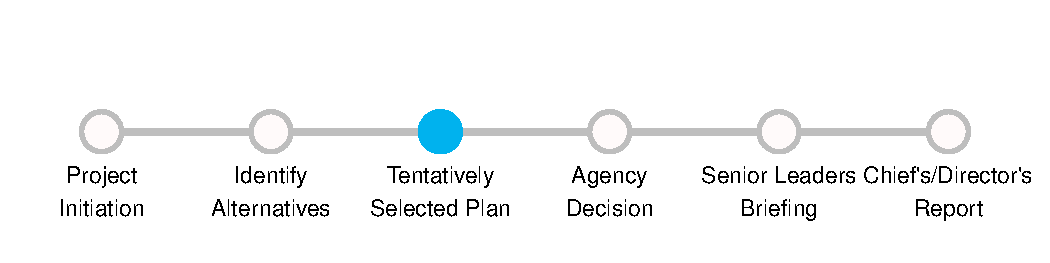
\includegraphics{RiskItemReport_files/figure-latex/milestoneplot-1} \end{center}

\hypertarget{lead-discipline-engineering---hydrology-and-hydraulics}{%
\subparagraph{\texorpdfstring{\textbf{Lead Discipline:} Engineering -
Hydrology and
Hydraulics}{Lead Discipline: Engineering - Hydrology and Hydraulics}}\label{lead-discipline-engineering---hydrology-and-hydraulics}}

\hypertarget{naccs-uses-save-points-throughout-boston-harbor-and-interpolates-those-data-points-across-the-terrain-showing-a-1d-result-of-where-the-water-ends-up-and-incorporates-slc-at-the-first-year-and-the-last-year-in-the-g2crm-planning-model.-will-the-model-provide-accurate-depiction-of-the-floodplain-extents-and-flood-pathway-entry-point-for-formulation-and-economic-analysis}{%
\subparagraph{NACCS uses save points throughout Boston Harbor and
interpolates those data points across the terrain showing a 1D result of
where the water ends up and incorporates SLC at the first year and the
last year in the G2CRM planning model. Will the model provide accurate
depiction of the floodplain extents and flood pathway entry point for
formulation and economic
analysis?}\label{naccs-uses-save-points-throughout-boston-harbor-and-interpolates-those-data-points-across-the-terrain-showing-a-1d-result-of-where-the-water-ends-up-and-incorporates-slc-at-the-first-year-and-the-last-year-in-the-g2crm-planning-model.-will-the-model-provide-accurate-depiction-of-the-floodplain-extents-and-flood-pathway-entry-point-for-formulation-and-economic-analysis}}

\begin{center}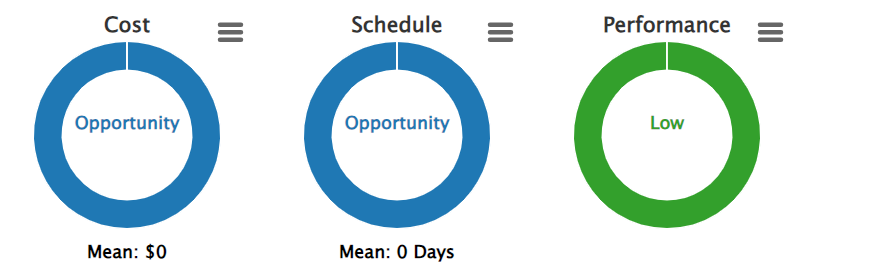
\includegraphics[width=12.1in]{images/montecarlo} \end{center}

\hypertarget{event-likelihood-likely-50-to-70}{%
\paragraph{\texorpdfstring{\textbf{Event Likelihood:} Likely (50\% to
70\%)}{Event Likelihood: Likely (50\% to 70\%)}}\label{event-likelihood-likely-50-to-70}}

\hypertarget{without-specific-refinement-and-updating-the-storm-suite-it-is-likely-that-the-model-will-not-accurately-reflect-extra-tropical-events-nor-will-it-have-the-refined-mesh-to-depict-an-accurate-floodplain-over-a-100-year-planning-horizon.}{%
\paragraph{Without specific refinement, and updating the storm suite, it
is likely that the model will not accurately reflect extra-tropical
events, nor will it have the refined mesh to depict an accurate
floodplain over a 100-year planning
horizon.}\label{without-specific-refinement-and-updating-the-storm-suite-it-is-likely-that-the-model-will-not-accurately-reflect-extra-tropical-events-nor-will-it-have-the-refined-mesh-to-depict-an-accurate-floodplain-over-a-100-year-planning-horizon.}}

\hypertarget{no-impact}{%
\paragraph{\texorpdfstring{\textbf{No
Impact}}{No Impact}}\label{no-impact}}

\begin{longtable}[]{@{}
  >{\raggedright\arraybackslash}p{(\columnwidth - 4\tabcolsep) * \real{0.2877}}
  >{\raggedright\arraybackslash}p{(\columnwidth - 4\tabcolsep) * \real{0.3425}}
  >{\raggedright\arraybackslash}p{(\columnwidth - 4\tabcolsep) * \real{0.3699}}@{}}
\toprule()
\begin{minipage}[b]{\linewidth}\raggedright
Cost Impact
\end{minipage} & \begin{minipage}[b]{\linewidth}\raggedright
Schedule Impact
\end{minipage} & \begin{minipage}[b]{\linewidth}\raggedright
Performance Impact
\end{minipage} \\
\midrule()
\endhead
No Cost Impact anticipated. & No Schedule Impact is Anticipated & No
Performance Impact is anticipated \\
\bottomrule()
\end{longtable}

\hypertarget{uniform-example}{%
\paragraph{\texorpdfstring{\textbf{Uniform
Example}}{Uniform Example}}\label{uniform-example}}

\begin{longtable}[]{@{}
  >{\raggedright\arraybackslash}p{(\columnwidth - 4\tabcolsep) * \real{0.2778}}
  >{\raggedright\arraybackslash}p{(\columnwidth - 4\tabcolsep) * \real{0.3194}}
  >{\raggedright\arraybackslash}p{(\columnwidth - 4\tabcolsep) * \real{0.4028}}@{}}
\toprule()
\begin{minipage}[b]{\linewidth}\raggedright
Cost Impact
\end{minipage} & \begin{minipage}[b]{\linewidth}\raggedright
Schedule Impact
\end{minipage} & \begin{minipage}[b]{\linewidth}\raggedright
Performance Impact
\end{minipage} \\
\midrule()
\endhead
\emph{Lowest} \$0 & \emph{Lowest} 0 days & \textbf{\emph{Performance
Impact:}} An inaccurate floodplain could result in reformulation;
significant redesign; post-authorization in the future. \\
\emph{Highest} \$0 & \emph{Highest} 0 days & \textbf{\emph{Performance
Impact Type:}} Other \\
NA & NA & An inaccurate floodplain could result in reformulation;
significant redesign; post-authorization in the future. \\
\bottomrule()
\end{longtable}

\begin{longtable}[]{@{}
  >{\raggedright\arraybackslash}p{(\columnwidth - 4\tabcolsep) * \real{0.2917}}
  >{\raggedright\arraybackslash}p{(\columnwidth - 4\tabcolsep) * \real{0.3333}}
  >{\raggedright\arraybackslash}p{(\columnwidth - 4\tabcolsep) * \real{0.3750}}@{}}
\toprule()
\begin{minipage}[b]{\linewidth}\raggedright
Cost Impact
\end{minipage} & \begin{minipage}[b]{\linewidth}\raggedright
Schedule Impact
\end{minipage} & \begin{minipage}[b]{\linewidth}\raggedright
Performance Impact
\end{minipage} \\
\midrule()
\endhead
\emph{Lowest} \$0 & \emph{Lowest} 0 days & \textbf{\emph{Performance
Impact:}} An inaccurate floodplain could result in reformulation;
significant redesign; post-authorization in the future. \\
\bottomrule()
\end{longtable}

\hypertarget{point-estimate-example}{%
\paragraph{\texorpdfstring{\textbf{Point Estimate
Example}}{Point Estimate Example}}\label{point-estimate-example}}

\begin{longtable}[]{@{}
  >{\raggedright\arraybackslash}p{(\columnwidth - 4\tabcolsep) * \real{0.2603}}
  >{\raggedright\arraybackslash}p{(\columnwidth - 4\tabcolsep) * \real{0.2603}}
  >{\raggedright\arraybackslash}p{(\columnwidth - 4\tabcolsep) * \real{0.4795}}@{}}
\toprule()
\begin{minipage}[b]{\linewidth}\raggedright
Cost Impact
\end{minipage} & \begin{minipage}[b]{\linewidth}\raggedright
Schedule Impact
\end{minipage} & \begin{minipage}[b]{\linewidth}\raggedright
Performance Impact
\end{minipage} \\
\midrule()
\endhead
Most Likely 0 & Most Likely 0 & \textbf{\emph{Performance Impact:}} An
inaccurate floodplain could result in reformulation; significant
redesign; post-authorization in the future. Performance Impact Type: \\
NA & NA & An inaccurate floodplain could result in reformulation;
significant redesign; post-authorization in the future. \\
\bottomrule()
\end{longtable}

\hypertarget{risk-treatments}{%
\subsection{Risk Treatments:}\label{risk-treatments}}

\begin{verbatim}
## Warning in add_header_above(., c(Measures = 2, Impacts = 2, Implemented = 1)):
## Please specify format in kable. kableExtra can customize either HTML or LaTeX
## outputs. See https://haozhu233.github.io/kableExtra/ for details.
\end{verbatim}

\begin{longtable}[]{@{}
  >{\raggedright\arraybackslash}p{(\columnwidth - 8\tabcolsep) * \real{0.0178}}
  >{\raggedright\arraybackslash}p{(\columnwidth - 8\tabcolsep) * \real{0.8817}}
  >{\centering\arraybackslash}p{(\columnwidth - 8\tabcolsep) * \real{0.0414}}
  >{\centering\arraybackslash}p{(\columnwidth - 8\tabcolsep) * \real{0.0178}}
  >{\centering\arraybackslash}p{(\columnwidth - 8\tabcolsep) * \real{0.0414}}@{}}
\toprule()
\endhead
1 & The risk can be mitigated working with ERDC prior to undergoing
detailed project modeling to refine the CHS Model specific to the Boston
Study Need. & 1e+05 & 0 &

\includegraphics{C:/workspace/e-rarr//RiskItemReportShinyApp/images/check.png} \\
2 & After the refinement, and existing/FWOP modeling is complete,
schedule an IPR with the Horizontal and Vertical Team to ensure
alignment on FWOP. & 0e+00 & 0 &

\includegraphics{C:/workspace/e-rarr//RiskItemReportShinyApp/images/check.png} \\
\bottomrule()
\end{longtable}

\hypertarget{risk-log}{%
\subsection{Risk Log:}\label{risk-log}}

\begin{verbatim}
## Warning in kable_styling(., bootstrap_options = c("striped", "hover",
## "condensed", : Please specify format in kable. kableExtra can customize either
## HTML or LaTeX outputs. See https://haozhu233.github.io/kableExtra/ for details.
\end{verbatim}

\begin{verbatim}
## Warning in column_spec(., 5, color = "black", background =
## risk_log_table$costcolor): Please specify format in kable. kableExtra can
## customize either HTML or LaTeX outputs. See
## https://haozhu233.github.io/kableExtra/ for details.
\end{verbatim}

\begin{verbatim}
## Warning in column_spec(., 6, color = "black", background =
## risk_log_table$schedulecolor): Please specify format in kable. kableExtra can
## customize either HTML or LaTeX outputs. See
## https://haozhu233.github.io/kableExtra/ for details.
\end{verbatim}

\begin{verbatim}
## Warning in column_spec(., 7, color = "black", background =
## risk_log_table$performancecolor): Please specify format in kable. kableExtra
## can customize either HTML or LaTeX outputs. See
## https://haozhu233.github.io/kableExtra/ for details.
\end{verbatim}

\begin{verbatim}
## Warning in column_spec(., 5:7, border_left = T, border_right = T): Please
## specify format in kable. kableExtra can customize either HTML or LaTeX outputs.
## See https://haozhu233.github.io/kableExtra/ for details.
\end{verbatim}

\begin{longtable}[]{@{}
  >{\raggedright\arraybackslash}p{(\columnwidth - 12\tabcolsep) * \real{0.0590}}
  >{\raggedright\arraybackslash}p{(\columnwidth - 12\tabcolsep) * \real{0.0852}}
  >{\raggedright\arraybackslash}p{(\columnwidth - 12\tabcolsep) * \real{0.5410}}
  >{\centering\arraybackslash}p{(\columnwidth - 12\tabcolsep) * \real{0.2197}}
  >{\centering\arraybackslash}p{(\columnwidth - 12\tabcolsep) * \real{0.0197}}
  >{\centering\arraybackslash}p{(\columnwidth - 12\tabcolsep) * \real{0.0328}}
  >{\centering\arraybackslash}p{(\columnwidth - 12\tabcolsep) * \real{0.0426}}@{}}
\toprule()
\begin{minipage}[b]{\linewidth}\raggedright
Edit Date
\end{minipage} & \begin{minipage}[b]{\linewidth}\raggedright
Reason for Change
\end{minipage} & \begin{minipage}[b]{\linewidth}\raggedright
Risk Log Note
\end{minipage} & \begin{minipage}[b]{\linewidth}\centering
Measures Implemented
\end{minipage} & \begin{minipage}[b]{\linewidth}\centering
Cost
\end{minipage} & \begin{minipage}[b]{\linewidth}\centering
Schedule
\end{minipage} & \begin{minipage}[b]{\linewidth}\centering
Performance
\end{minipage} \\
\midrule()
\endhead
1/30/2023 4:02 PM & New Project Risk & New Risk Added &

\includegraphics{C:/workspace/e-rarr//RiskItemReportShinyApp/images/check.png}
& 1 & 1 & 2 \\
1/30/2023 4:05 PM & New Information & If I don't keep saving updates,
the program times out on me. &

\includegraphics{C:/workspace/e-rarr//RiskItemReportShinyApp/images/check.png}
& 0 & 0 & 3 \\
1/30/2023 4:07 PM & New Information & Updating Risk &

\includegraphics{C:/workspace/e-rarr//RiskItemReportShinyApp/images/check.png}
& 0 & 0 & 3 \\
1/30/2023 4:10 PM & New Information & Updating Risk &

\includegraphics{C:/workspace/e-rarr//RiskItemReportShinyApp/images/check.png}
& 0 & 0 & 3 \\
2/14/2023 7:48 PM & New Information & NA &

\includegraphics{C:/workspace/e-rarr//RiskItemReportShinyApp/images/check.png}
& 0 & 0 & 3 \\
3/23/2023 7:41 PM & Risk Response implemented & 15 March an IPR was held
with HH\&C CoP, L\&PC Team, MSC, and PCX to discuss modeling strategy.
17 March, the Chief of Planning at NAD approved the modeling strategy. &
\includegraphics{NA} & 0 & 0 & 3 \\
3/24/2023 2:17 PM & Corrected Error & NA & \includegraphics{NA} & 0 & 0
& 3 \\
\bottomrule()
\end{longtable}

\end{document}
